\documentclass{article}
\usepackage{amsmath, amssymb, amsthm, enumerate, graphicx}
\usepackage[usenames,dvipsnames]{color}
\usepackage{bm}
\usepackage[colorlinks=true,urlcolor=blue]{hyperref}
\usepackage{geometry}
\geometry{margin=1in}
\usepackage{float}
\usepackage{graphics}
\setlength{\marginparwidth}{2.15cm}
\usepackage{booktabs}
\usepackage{enumitem}
\usepackage{epsfig}
\usepackage{setspace}
\usepackage{parskip}
\usepackage{enumerate}
\usepackage[normalem]{ulem}
\usepackage{tikz}
\usetikzlibrary{positioning, arrows, automata}
\usepackage{pgfplots}
\usepackage[font=scriptsize]{subcaption}
\usepackage{float}
\usepackage[]{algorithm2e}
\usepackage{environ}
\usepackage{bbm}
\usepackage{graphicx}
\usepackage{titling}
\usepackage{url}
\usepackage{color}
\usepackage{xcolor}
\usepackage{lipsum}
\usepackage{lastpage}
\usepackage[colorlinks=true,urlcolor=blue]{hyperref}
\usepackage{multicol}
\usepackage{tabularx}
\usepackage{comment}
\usepackage[utf8]{inputenc}
\usepackage{amssymb}
\usepackage{setspace}
\usepackage{marvosym}
\usepackage{wrapfig}
\usepackage{datetime}
\usepackage[many]{tcolorbox}
\usepackage{array}
\usepackage{multirow}
\usepackage{wasysym}
\usepackage{cancel}
\usepackage{framed}
\usepackage{dsfont}

\usepackage{listings}
\usepackage{color}

% Define all course dates in a single file
% ===========================================================================
% 10-701 Course Dates Configuration File
% ===========================================================================
\newcommand{\currentsemester}{Fall 2026}

% ---------------------------------------------------------------------------
% Homework Dates
% ---------------------------------------------------------------------------

% Homework 1
\newcommand{\hwOneRelease}{Friday, Aug. 28, 2026}
\newcommand{\hwOneDue}{Tuesday, Sep. 8, 2026}

% Define all course links in a single file
\usepackage{hyperref}

\newcommand{\DeclarePlainURL}[1]{%
  \begingroup
  \catcode35=12 % #
  \catcode37=12 % percent sign
  \catcode38=12 % &
  \catcode94=12 % ^
  \catcode95=12 % _
  \catcode126=12 % ~
  \DeclarePlainURLAux#1%
}

\def\DeclarePlainURLAux#1#2{%
  \endgroup
  \def#1{#2}%
}

\urldef{\currentpiazza}\url{https://piazza.com/cmu/fall2026/10701/home}
\DeclarePlainURL{\currentsyllabus}{https://10-701.github.io/index.html#Syllabus}


\newcommand{\R}{\mathbb{R}}
\newcommand{\blackcircle}{\tikz\draw[black,fill=black] (0,0) circle (1ex);}
\renewcommand{\circle}{\tikz\draw[black] (0,0) circle (1ex);}
\newcommand{\eMLE}{\widehat{\theta}_{\text{MLE}}}


\newtcolorbox[]{your_solution}[1][]{
    % breakable,
    enhanced,
    nobeforeafter,
    colback=white,
    title=Your Answer,
    sidebyside align=top,
    box align=top,
    #1
}

% Custom functions
\newcommand{\vind}[1]{\mathbbm{1}_{#1}}
\newcommand{\Lagr}{\mathcal{L}}


% SOLUTION environment
\NewEnviron{soln}{
\leavevmode\color{red}\ignorespaces \textbf{Solution} \BODY }{}

% QUESTION AUTHORS environment
\NewEnviron{qauthor}{
\leavevmode\color{blue}\ignorespaces \textbf{Author} \BODY}{}

% TO ONLY SHOW HOMEWORK QUESTIONS, include following (else comment out):
% \RenewEnviron{soln}{}
% \RenewEnviron{qauthor}{}



\makeatletter
\newcommand{\removelatexerror}{\let\@latex@error\@gobble}
\makeatother

\newcommand{\argmax}{\mathop{\mathrm{argmax}}}
\newcommand{\argmin}{\mathop{\mathrm{argmin}}}

\pgfplotsset{compat=1.17}

%%%%%%%%%%%%%%%%%%%%%%%%%%%%%%%%%%%%%%%%%%%
% Code highlighting with listings         %
%%%%%%%%%%%%%%%%%%%%%%%%%%%%%%%%%%%%%%%%%%%

\definecolor{bluekeywords}{rgb}{0.13,0.13,1}
\definecolor{greencomments}{rgb}{0,0.5,0}
\definecolor{redstrings}{rgb}{0.9,0,0}
\definecolor{light-gray}{gray}{0.95}

\newcommand{\MYhref}[3][blue]{\href{#2}{\color{#1}{#3}}}%

\definecolor{dkgreen}{rgb}{0,0.6,0}
\definecolor{gray}{rgb}{0.5,0.5,0.5}
\definecolor{mauve}{rgb}{0.58,0,0.82}

\lstdefinelanguage{Shell}{
  keywords={tar, cd, make},
  %keywordstyle=\color{bluekeywords}\bfseries,
  alsoletter={+},
  ndkeywords={python, py, javac, java, gcc, c, g++, cpp, .txt, octave, m, .tar},
  %ndkeywordstyle=\color{bluekeywords}\bfseries,
  identifierstyle=\color{black},
  sensitive=false,
  comment=[l]{//},
  morecomment=[s]{/*}{*/},
  commentstyle=\color{purple}\ttfamily,
  stringstyle=\color{red}\ttfamily,
  morestring=[b]',
  morestring=[b]",
  backgroundcolor = \color{light-gray}
}

\lstset{columns=fixed, basicstyle=\ttfamily,
    backgroundcolor=\color{light-gray},xleftmargin=0.5cm,frame=tlbr,framesep=4pt,framerule=0pt,
    showstringspaces=false}

%%%%%%%%%%%%%%%%%%%%%%%%%%%%%%%%%%%%%%%%%%%
% Custom box for highlights               %
%%%%%%%%%%%%%%%%%%%%%%%%%%%%%%%%%%%%%%%%%%%

% Define box and box title style
\tikzstyle{mybox} = [fill=blue!10, very thick,
    rectangle, rounded corners, inner sep=1em, inner ysep=1em]


\NewEnviron{notebox}{

\begin{tikzpicture}
\node [mybox] (box){
    \begin{minipage}{\textwidth}
        \BODY
    \end{minipage}
};
\end{tikzpicture}
}

%%%%%%%%%%%%%%%%%%%%%%%%%%%%%%%%%%%%%%%%%%%
% Matchy self-defined commands            %
%%%%%%%%%%%%%%%%%%%%%%%%%%%%%%%%%%%%%%%%%%%

\DeclareRobustCommand{\answerfont}{%
  \fontencoding{T1}%
  \fontfamily{LinuxLibertineT-LF}%
  \selectfont
}

\newenvironment{answer}
  {\par\begingroup\answerfont}
  {\par\endgroup}

\DeclareRobustCommand{\ans}[1]{%
  {\answerfont #1}%
}


\begin{document}
\section*{}
\begin{center}
  \centerline{\textsc{\LARGE  Homework 1}}
  \vspace{0.5em}
  \centerline{\textsc{\LARGE Overfitting and Decision Trees}\footnote{Compiled on \today{} at \currenttime{}}}
  \vspace{1em}
  \textsc{\large CMU 10-701: Introduction to Machine Learning (\currentsemester)} \\
  \vspace{0.5em}
  \currentpiazza \\
  \vspace{0.5em}
  \centerline{OUT: \hwOneRelease}
  %\today{} at \currenttime{}}}
  \vspace{0.5em}
  \centerline{DUE: \hwOneDue, 11:59pm}
\end{center}

\section*{START HERE: Instructions}
\begin{itemize}
\item \textbf{Collaboration policy:} Collaboration on solving the homework is allowed, after you have thought about the problems on your own. It is also OK to get clarification (but not solutions) from books or online resources, again after you have thought about the problems on your own. There are two requirements: first, cite your collaborators fully and completely (e.g., ``Jane explained to me what is asked in Question 2.1''). Second, write your solution {\em independently}: close the book and all of your notes, and send collaborators out of the room, so that the solution comes from you only. See the Academic Integrity Section in our \href{\currentsyllabus}{Course Syllabus} for more information.

\item\textbf{Late Submission Policy:} See the late homework policy in our \href{\currentsyllabus}{Course Syllabus}

\item\textbf{Submitting your work:}

\begin{itemize}

\item \textbf{Gradescope:} There will be two submission slots for this homework on Gradescope: Written and Programming. \\
For the written problems such as short answer, multiple choice, derivations, proofs, or plots, we will be using the written submission slot. Please use the provided template. The best way to format your homework is by using the Latex template released in the handout and writing your solutions in Latex. However submissions can be handwritten onto the template, but should be labeled and clearly legible. If your writing is not legible, you will not be awarded marks.  Each derivation/proof should be  completed in the boxes provided below the question, \textbf{you should not move or change the sizes of these boxes} as Gradescope is expecting your solved homework PDF to match the template on Gradescope. If you find you need more space than the box provides you should consider cutting your solution down to its relevant parts, if you see no way to do this, please add an additional page at the end of the homework and guide us there with a 'See page xx for the rest of the solution'.\\
You are also required to upload your code, which you wrote to solve the final question of this homework, to the Programming submission slot. Your code may be run by TAs so please make sure it is in a workable state.\\
Regrade requests can be made after the homework grades are released, however this gives the TA the opportunity to regrade your entire paper, meaning if additional mistakes are found then points will be deducted.
\end{itemize}

\end{itemize}

For multiple choice or select all that apply questions, shade in the box or circle in the template document corresponding to the correct answer(s) for each of the questions. For \LaTeX users, use $\blacksquare$ and \blackcircle  for shaded boxes and circles, and don't change anything else. If an answer box is included for showing work, \textbf{you must show your work}!



\clearpage


\section{Overfitting in 1D}
Scotty just learned how a linear binary classifier for  $\mathbb{R}$ works. The binary labels are $\{-,+\}$. A linear classifier $C: \mathbb{R} \to \{-,+\}$ determines the label $C(x)$ associated with any $x \in \mathbb{R}$. In $\mathbb{R}$, a classifier is a linear classifier if and only if it can be formulated as follows: 
\[
C(x) = \begin{cases}
    + \text{ if } wx + b \geq 0 \\
    - \text{ else}
\end{cases}
\]
where $w, b \in \mathbb{R}$ are fixed. \\
\\
Scotty is currently on vacation in a 1d world. He walks along a path in $\mathbb{R}$. There are two points $x^{(1)},x^{(2)}$ at positions $-1$ and $1$ respectively. 


\begin{center}
    \begin{tikzpicture}
        \draw[->] (-3, 0) -- (3,0) node[right] {$\mathbb{R}$};
        \filldraw (-1,0) circle (2pt) node[below=3pt] {$x^{(1)}$};
        \filldraw (1,0) circle (2pt) node[below=3pt] {$x^{(2)}$};
    
        \node[above=3pt] at (-1,0) {$-1$};
        \node[above=3pt] at (1,0) {$1$};
    \end{tikzpicture}
\end{center}


Scotty has a metal detector and is trying to see if there is treasure at positions $x^{(1)},x^{(2)}$. \\
A label of ``$-$" indicates no treasure, and ``$+$" indicates treasure. In the true, unknown state of the world, there is gold under $x^{(2)}$ but no gold at $x^{(1)}$. The true label for $x^{(1)}$ is $``-"$ and for $x^{(2)}$ is $``+"$. \\
\\
Scotty trains a linear model to determine where there is treasure or not. However, there is noise and the metal detector is not always accurate. Let $\alpha \in [0,1]$ be the noise factor. The metal detector returns the wrong label with probability $\frac{\alpha}{2}$, independently for each measurement. (So, we can think of $\alpha$ as the probability that we replace the true label by uninformative (uniform) noise.) The probabilities are shown in the following table:


\begin{table}[h]
    \centering
    \caption{Metal detector result probability}
    \begin{tabular}{||c|cc||}
    \hline
        ~ & $x^{(1)}$ & $x^{(2)}$ \\ \hline \hline
        $-$ & $1-\frac{\alpha}{2}$ & $\frac{\alpha}{2}$ \\ \hline
        $+$ & $\frac{\alpha}{2}$ & $1-\frac{\alpha}{2}$ \\ \hline
    \end{tabular}
\end{table}

Scotty wants to use 0-1 loss: the penalty of incorrectly predicting a value is $1$;  in other words: 
\[L(y,\hat{y}) = \mathds{1} [y \neq \hat{y}]\]
Scotty gets two (statistically independent) readings, one from $x^{(1)}$ and one from $x^{(2)}$, which he uses as training data. He uses the training data to create a classifier that minimises the loss (with respect to training data). \\
\\
\begin{enumerate}

\item {\bf [2 points]} Training means picking a linear binary classifier that scores best on the \textbf{training} data. Using only two points $x^{(1)},x^{(2)}$, for training, there are only 4 unique classifiers that Scotty can pick. We will treat classifiers that induce the same labels on the same points as the same classifier. The outputs are shown the the rows of the table below. Fill in the probability that Scotty will pick each of these classifiers (with respect to the randomness in the training data). Leave answer in terms of $\alpha$.
\begin{table}[ht]
\begin{center}
\begin{tabular}{||c c c||} 
 \hline
 Label of $x^{(1)}$ & Label of $x^{(2)}$ & Probability  \\ [0.5ex] 
 \hline\hline
 + & +  & \\ 
 \hline
 + & $-$ & \\
 \hline
 $-$ & + &  \\
 \hline
 $-$ & $-$ &\\
 \hline
\end{tabular}
\end{center}
\end{table}


\item {\bf [2 points]}
To generate a test set, Scotty collects another observation randomly with equal probability from $x^{(1)}$ or $x^{(2)}$. The metal detector's probability outputs remain the same as before. \\
For each of the four classifiers, compute the expected error on this new example (i.e., the expected test error). Leave the answer as a function of $\alpha$.
\begin{tcolorbox}[fit,height=5cm, width=0.9\textwidth, blank, borderline={1pt}{-2pt}]
\end{tcolorbox}


\item {\bf [2 points]}
What is the expected test error averaged over the randomness in the training set? Give your answer in terms of $\alpha$.
\begin{tcolorbox}[fit,height=2.5cm, width=0.9\textwidth, blank, borderline={1pt}{-2pt}]
\end{tcolorbox}

\newpage

\item {\bf [4 points]}
Create a plot that shows three lines:
\begin{itemize}
    \item the expected test error at $\alpha\in \{0.0, 0.25, 0.5, 0.75, 1.0\}$
    \item the minimum possible test error at these same values of $\alpha$ — in other words, the error if Scotty knew the correct classifier ahead of time, and evaluated it on a newly sampled test example.
    \item the expected training error at these same values of $\alpha$.
\end{itemize}

\begin{tcolorbox}[fit,height=12cm, width=0.9\textwidth, blank, borderline={1pt}{-2pt}]
\end{tcolorbox}


\item {\bf [2 points]}
The difference between the first and second lines in \textbf{part 4} is one possible measure of the amount of overfitting: the expected excess test error because our training process has to work from a limited-size, noisy training set. Similarly, the difference between the first and third lines in \textbf{part 4} is another measure: the expected optimism when comparing training to test error. At what $\alpha$ value is overfitting the worst according to each of these measures? Why?

\begin{tcolorbox}[fit,height=5cm, width=0.9\textwidth, blank, borderline={1pt}{-2pt}]
\end{tcolorbox}


\end{enumerate}

\newpage

\section{Repeating the Overfitting Analysis in Two Dimensions}

Scotty now visits a two-dimensional world. For a point $x=(x_1,x_2)$, an
affine linear classifier has the form
\[
C_{\mathbf{w},b}(x)=
\begin{cases}
+, & w_1x_1+w_2x_2+b\geq 0,\\
-, & w_1x_1+w_2x_2+b<0,
\end{cases}
\]
where $\mathbf{w}=(w_1,w_2)\neq(0,0)$ and $b\in\mathbb{R}$.

Consider the following two sets of points, where $S_3$ consists of three
vertices of a square and $S_4$ consists of all four vertices:
\[
\begin{aligned}
S_3 &= \{x^{(1)}=(-1,-1),\ x^{(2)}=(-1,1),\ x^{(3)}=(1,1)\},\\
S_4 &= \{x^{(1)}=(-1,-1),\ x^{(2)}=(-1,1),\ x^{(3)}=(1,1),
        \ x^{(4)}=(1,-1)\}.
\end{aligned}
\]
The noise-free labels are determined by the vertical linear classifier
\[
f^*(x)=
\begin{cases}
-, & x_1<0,\\
+, & x_1>0.
\end{cases}
\]
Thus, in the point order displayed above, the noise-free label vectors are
$(-,-,+)$ for $S_3$ and $(-,-,+,+)$ for $S_4$.

As in Question 1, Scotty observes one noisy training label at every point. For
each point independently, with probability $\alpha\in[0,1]$, the noise process
\emph{replaces} its noise-free label with the result of a fair coin flip; with
probability $1-\alpha$, the noise-free label is retained. Therefore
\[
\Pr(\text{observed label is correct})=1-\frac{\alpha}{2},
\qquad
\Pr(\text{observed label is incorrect})=\frac{\alpha}{2}.
\]
In particular, when $\alpha=1$, the observed label is equally likely to be
$+$ or $-$, regardless of the noise-free label. For convenience, define
\[
q=\frac{\alpha}{2}.
\]

Scotty chooses an affine linear classifier that minimizes its average 0--1
loss on the training set. Again, classifiers that induce the same labels on
the finite point set are treated as one classifier. If several distinct
induced labelings attain the same minimum training error, Scotty chooses
uniformly at random among them. This tie-breaking rule is important for $S_4$.

To obtain a test example, first choose a point uniformly from $S_m$ and then
obtain a new, independent label using the same replacement-noise process and
the same value of $\alpha$. In particular, the test label is independent of
the training label conditional on the selected point.

\begin{enumerate}
\renewcommand{\labelenumi}{\textbf{(\alph{enumi})}}
\setlength{\itemsep}{1.5em}

\item {\bf [2 points]}
For each of $S_3$ and $S_4$, how many of the possible binary labelings are
realizable by an affine linear classifier?  Identify any non-realizable
labelings and explain geometrically why a straight line cannot separate their
positive and negative points.
\begin{tcolorbox}[height=4cm, width=\linewidth]

\end{tcolorbox}

\item {\bf [2 points]}
Compute the probability that Scotty learns each possible classifier on $S_3$
and $S_4$.  To avoid listing every classifier separately, group learned
labelings by their Hamming distance $k$ from the noise-free label vector.  In
your table, report (i) the number of learned labelings in each group and (ii)
the probability of learning \emph{each individual labeling} in that group.
Be careful to distinguish the probability of \emph{observing} a particular
training labeling from the probability of \emph{learning} a classifier that
induces that labeling on the point set.
\begin{tcolorbox}[height=7cm, width=\linewidth]

\end{tcolorbox}

\item {\bf [2 points]}
Suppose a learned classifier disagrees with the noise-free label vector at
exactly $k$ of the $m$ points in $S_m$.  Compute its expected test error as a
function of $k$, $m$, and $\alpha$.
\begin{tcolorbox}[height=4cm, width=\linewidth]

\end{tcolorbox}


\item {\bf [2 points]}
Average over the randomness in the training data and Scotty's tie-breaking.
For both $S_3$ and $S_4$, compute (i) the expected training error and (ii) the
expected test error.
\begin{tcolorbox}[height=5cm, width=\linewidth]

\end{tcolorbox}

\item {\bf [4 points]}
Make two plots, one for $S_3$ and one for $S_4$. On each plot, show:
\begin{itemize}
    \item the expected test error at $\alpha\in\{0,0.25,0.5,0.75,1\}$.
    \item the minimum possible expected test error at each of these $\alpha$ values for an oracle that knows $f^*$. 
    \item the expected training error at each $\alpha$.
\end{itemize}
Where is overfitting the worst, according to the difference between the first and second lines, and the difference between the first and third lines?

\begin{tcolorbox}[height=6cm, width=\linewidth]

\end{tcolorbox}



\item {\bf [3 points]}
You probably noticed that, on $S_4$, Scotty sometimes obtains strictly positive
training error, unlike the earlier setups.  Qualitatively, how does the
analysis change if we replace affine linear classifiers with a more expressive
hypothesis class that can realize all $16$ labelings of $S_4$ and therefore
always attain zero training error?  What happens to our measures of overfitting?
\begin{tcolorbox}[height=5cm, width=\linewidth]

\end{tcolorbox}



\end{enumerate}




\newpage

\clearpage
\section{Decision Trees [20 pts]}
\begin{enumerate}


\item Consider the dataset in Table \ref{dec_tab} for this problem. Given the four attributes on the left, we want to predict if the student got an A in the course. The following questions involve some computation, so you may want to solve them programmatically. You can find this dataset in \textit{data.txt}

\begin{table}[ht]
\begin{center}
\begin{tabular}{| c | c | c | c || c |} 
\hline
\vtop{\hbox{\strut \textbf{Wakes Up}}\hbox{\strut \textbf{Early}}} & \vtop{\hbox{\strut \textbf{Finished All}}\hbox{\strut \textbf{Homework}}} & \vtop{\hbox{\strut \textbf{Completed}}\hbox{\strut \textbf{Pre-requisites}}} & \textbf{Likes Coffee} & \textbf{A} \\ 
\hline
1 & 1 & 0 & 0 & 0\\ 
\hline
1 & 1 & 1 & 0 & 1\\ 
\hline
0 & 0 & 1 & 0 & 0\\ 
\hline
0 & 1 & 1 & 0 & 1\\ 
\hline
0 & 1 & 1 & 0 & 1\\ 
\hline
0 & 0 & 1 & 1 & 0\\ 
\hline
1 & 0 & 0 & 0 & 0\\ 
\hline
0 & 1 & 0 & 1 & 1\\ 
\hline
0 & 0 & 1 & 0 & 1\\ 
\hline
1 & 0 & 0 & 0 & 0\\ 
\hline
1 & 1 & 1 & 0 & 1\\ 
\hline
0 & 1 & 1 & 1 & 0\\ 
\hline
0 & 0 & 0 & 0 & 0\\ 
\hline
1 & 0 & 0 & 1 & 0\\ 
\hline
\end{tabular}
\end{center}
\caption{decision tree features and labels}
\label{dec_tab}
\end{table}

Create a decision tree of depth 2 using the ID3 algorithm from class. The tree should have the same structure as the diagram in Figure~\ref{fig:tree}. Note that 0 leads to the left branch and 1 leads to the right branch. 
\begin{figure}[ht]
\begin{center}
  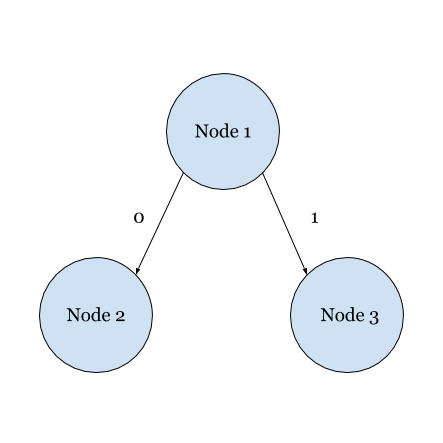
\includegraphics[width=5cm]{images/decisiontree.png}
\end{center}
  \caption{Decision tree structure for question 1}
\label{fig:tree}
\end{figure}
\begin{enumerate}[label=(\roman*)]

\newpage

\item \textbf{[2 pts]} What is the attribute at Node 1? What is the information gain of this attribute? Please round your answer to 4 decimal places.

Attribute to split on: \begin{tcolorbox}[fit,height=1.2cm, width=3.5cm, blank, borderline={1pt}{-2pt}, nobeforeafter, box align = center] \end{tcolorbox}
\hspace{0.5cm} Mutual information: \begin{tcolorbox}[fit,height=1.2cm, width=3.5cm, blank, borderline={1pt}{-2pt}, nobeforeafter, box align = center] \end{tcolorbox} 
 
    
\item \textbf{[2 pts]} What is the attribute at Node 2? What is the information gain of this attribute? Please round your answer to 4 decimal places.

Attribute to split on: \begin{tcolorbox}[fit,height=1.2cm, width=3.5cm, blank, borderline={1pt}{-2pt}, nobeforeafter, box align = center] \end{tcolorbox}
\hspace{0.5cm} Mutual information: \begin{tcolorbox}[fit,height=1.2cm, width=3.5cm, blank, borderline={1pt}{-2pt}, nobeforeafter, box align = center] \end{tcolorbox} 



\item \textbf{[2 pts]} What is the attribute at Node 3? What is the information gain of this attribute? Please round your answer to 4 decimal places. \\
\\
Note: If there is a tie on the attribute with the highest information gain, write any of the attribute that has the highest information gain.

Attribute to split on: \begin{tcolorbox}[fit,height=1.2cm, width=3.5cm, blank, borderline={1pt}{-2pt}, nobeforeafter, box align = center] \end{tcolorbox}
\hspace{0.5cm} Mutual information: \begin{tcolorbox}[fit,height=1.2cm, width=3.5cm, blank, borderline={1pt}{-2pt}, nobeforeafter, box align = center] \end{tcolorbox} 


    
\end{enumerate}

\item \textbf{[4 pts]} Consider learning a decision tree for some binary classification task. Assume that we do not restrict the size of the tree and that the tree can branch multiple times on the same attribute. Under what condition(s) would we be unable to construct a tree that perfectly classifies the dataset?  
\begin{tcolorbox}[fit,height=5cm, width=15cm, blank, borderline={1pt}{-2pt}]
\end{tcolorbox}


\item \textbf{[4 pts]} Assuming that there are no inconsistencies in the data, is the ID3 algorithm guaranteed to output the smallest decision tree that can perfectly classify the training data i.e., achieves zero training error rate? Briefly explain why or why not. \\
\textit{Note:} Inconsistent data is when there are at least two data points $x^{(i)}$ and $x^{(j)}$ with identical feature values, such that $y^{(i)} \neq y^{(j)}$.
\begin{tcolorbox}[fit,height=5cm, width=15cm, blank, borderline={1pt}{-2pt}]
%solution
\end{tcolorbox}


\newpage
\item {\bf [6 Points]} Recall that the information gain of some variable $A$ is the expected reduction in entropy of a target variable $Y$ in some dataset $S$ due to partitioning on $A$. Prove that information gain is always non-negative. To receive full credit, you must show all steps of your work. \textbf{Hint: }You may find the result proved in Recitation 1 regarding the \emph{KL divergence} between two distributions useful for this question.

        \begin{tcolorbox}[fit,height=19cm, width=0.95\textwidth, blank, borderline={1pt}{-2pt}]
  

        \end{tcolorbox}

\end{enumerate}
\newpage

\newpage
\clearpage
\input{programming_dt}
\clearpage
\section{Collaboration Questions}

\begin{enumerate}
    \item
    \begin{enumerate}
        \item Did you receive any help whatsoever from anyone in solving this assignment?

        \item If you answered `yes', give full details (e.g. “Jane Doe explained to me what is asked in Question 3.4”)\\

        \begin{tcolorbox}[fit,height=4cm, width=15cm, blank, borderline={1pt}{-2pt},nobeforeafter]

        I used generative AI to help me understand and implement some visualization code. To be specific:
            \begin{itemize}
                \item For Q2(a), I asked Claude Fable 5.1 to explain the definition of realizable, $S_3$ and $S_4$. I also asked a friend (Tesla Zhang, who is a PhD student in CSD but not taking this course) the same question.
            \end{itemize}

        \end{tcolorbox}

    \end{enumerate}


    \item
    \begin{enumerate}
        \item Did you give any help whatsoever to anyone in solving this assignment?


        \item If you answered `yes', give full details (e.g. “I pointed Joe Smith to section 2.3 since he didn’t know how to proceed with Question 2”)\\

        \begin{tcolorbox}[fit,height=4cm, width=15cm, blank, borderline={1pt}{-2pt},nobeforeafter]


        \end{tcolorbox}

    \end{enumerate}

    \item
    \begin{enumerate}
        \item Did you find or come across code that implements any part of this assignment?

        \item If you answered `yes', give full details (book \& page, URL \& location within the page, etc.).\\

        \begin{tcolorbox}[fit,height=4cm, width=15cm, blank, borderline={1pt}{-2pt},nobeforeafter]


        \end{tcolorbox}

    \end{enumerate}
\end{enumerate}



\end{document}
